\documentclass[10pt,aspectratio=169]{beamer}

\usepackage[T1]{fontenc}
\usepackage{lmodern}

\usepackage{amsmath,amssymb}
\usepackage{bm}
\usepackage{graphicx}
\usepackage{hyperref}
\usepackage{xcolor}
\usepackage{tikz}

\graphicspath{{./figures/}}

\title{Bayesian analysis and naturalness of (Next-to-)Minimal SUSY Models}

\author{D.~Harries\\
  {\scriptsize
    (IPNP, Charles University in Prague)}\\
  \vspace{25pt}
  { \scriptsize
    Based on: \href{https://doi.org/10.1007/JHEP10(2017)160}{%
      P.~Athron, C.~Bal\'{a}zs, B.~Farmer, A.~Fowlie, D.~Harries,
      and D.~Kim, JHEP \textbf{10}, 160 (2017)}
    [\href{http://arxiv.org/abs/1709.07895}{arXiv:1709.07895}]
  }
}

\titlegraphic{
  \begin{center}
    \hspace*{\fill}
    \includegraphics[scale=0.3]{uk_logo}
    \hspace*{\fill}
  \end{center}
}

\date[Phenomenology 2018, University of Pittsburgh]{May 7, 2018}

\usetheme{CambridgeUS}

\setbeamertemplate{headline}[default]{}
\setbeamertemplate{footline}[page number]{}
\setbeamertemplate{navigation symbols}{}

\begin{document}

\begin{frame}[plain]
  \titlepage
\end{frame}

\section{Naturalness Measures}

\begin{frame}
  \frametitle{Naturalness Problems}
  \begin{columns}[t]
    \begin{column}{0.5\textwidth}
      \begin{itemize} \itemsep1em
        \item Common motivation for SUSY is the hierarchy problem,
      \end{itemize}
      \begin{center}
        \includegraphics[width=0.8\textwidth]{fermionloop}
      \end{center}
      \begin{itemize} \itemsep1em
      \item Example of a \alert{``naturalness problem''}
        \begin{itemize}
        \item See also: strong CP problem, cosmological constant
          problem, flatness problem, $\ldots$
        \end{itemize}
      \end{itemize}
    \end{column}
    \begin{column}{0.5\textwidth}
      \begin{itemize} \itemsep1.5em
      \item Possible characterisation: {\color{blue} propensity of model to
        reproduce data}
      \item Related to \alert{fine-tuning}, e.g., if observations require
        a priori unjustified tuning of parameters $\Rightarrow$ model
        unnatural
      \item Prefer models in which fine-tuning not required/reduced?
      \item E.g., ``little hierarchy problem'' in MSSM
        (at tree-level)
        \begin{equation*}
          m_{h_1}^2 \leq m_Z^2 \cos^2 2\beta \, { \color{red} \lesssim
            (91 \text{ GeV})^2}
        \end{equation*}
        {\color{blue} $\Rightarrow$ non-minimal SUSY models?}
      \end{itemize}
    \end{column}
  \end{columns}
\end{frame}

\begin{frame}
  \frametitle{Quantifying Fine-tuning}
  \begin{block}{Typical Motivation}
    <model name> raises the Higgs mass at tree-level, and
    therefore is more natural than the MSSM, e.g., in the NMSSM
    \begin{equation*}
      m_{h_1}^2 \lesssim m_Z^2 \cos^2 2\beta + \frac{\lambda^2 v^2}{2}
      \sin^2 2\beta
    \end{equation*}
  \end{block}
  \begin{itemize} \itemsep1em
  \item Justify/check claim that model is more natural than another
    $\Rightarrow$ quantify naturalness, i.e., fine-tuning
  \item Traditionally, construct {\color{blue} fine-tuning measure}, i.e.,
    calculable function of model parameters that is identified with tuning
  \item Focus on different features of a model's behaviour $\Rightarrow$
    different fine-tuning measure
    \begin{itemize}
    \item Model fine-tuned according to one measure $\Rightarrow$ also
      fine-tuned under a different measure?
    \end{itemize}
  \item \alert{I.e., depends on your definition of fine-tuning $\ldots$}
  \end{itemize}
\end{frame}

\begin{frame}
  \frametitle{Traditional Tuning Measures}
  \begin{center}
    What constitutes "fine-tuning"? \\
    Opinions differ.
  \end{center}
  \begin{itemize} \itemsep0.8em
    \item Large cancellations?
      \begin{equation*}
        \Delta_{EW} = \max_i \frac{2|C_i|}{m_Z^2}, \quad C_1 = -\mu^2, \,
        C_2 = \frac{m_{H_d}^2}{\tan^2\beta - 1}, \ldots
      \end{equation*}
    \item Extreme sensitivities?
      \begin{equation*}
        \Delta_{BG} = \max_i \left | \frac{\partial \ln m_Z^2}
        {\partial \ln p_i} \right | , \quad p_i \in \{\text{fundamental
        parameters}\}
      \end{equation*}
    \item High or low energy contributions ($\Delta_{EW}$ or $\Delta_{HS}$)?
      Definition of parameters $p_i$? Just $m_Z$?
    \item Model fine-tuned $\Leftrightarrow \Delta_{EW/HS/BG/\ldots} > ?$
    \item Compare tuning between models?
  \end{itemize}
  \begin{center}
  \alert{What does $\Delta_{EW/HS/BC/\ldots} > x$ mean for our degree of belief
    in model?}
  \end{center}
\end{frame}

\begin{frame}
  \frametitle{Traditional Tuning Measures}
  \begin{columns}[t]
    \begin{column}{0.5\textwidth}
      \begin{figure}
        \centering
        \includegraphics[width=\textwidth]{msugra_measures_comparison}
      \end{figure}
    \end{column}
    \begin{column}{0.5\textwidth}
      \begin{figure}
        \centering
        \includegraphics[width=\textwidth]{nuhm2_measures_comparison}
      \end{figure}
    \end{column}
  \end{columns}
  \begin{center}
    \tiny
        [\href{http://arxiv.org/abs/1309.2984}{arXiv:1309.2984}]
  \end{center}
\end{frame}

\section{Bayesian Naturalness}

\begin{frame}
  \frametitle{A Bayesian Approach}
  \begin{itemize} \itemsep1.1em
  \item Results based on traditional measures depend heavily on
    choice of measure
  \item Generally, when we talk about ``naturalness'' we are really
    talking about plausibility
    \begin{itemize} \itemsep0.8em
    \item Unnatural model $\Leftrightarrow$ implausible model
    \item \alert{Traditional measures do not have an unambiguous interpretation
      in this sense}
    \end{itemize}
  \item $\Rightarrow$ better questions to ask are,
    \vspace{7pt}
    \begin{center}
      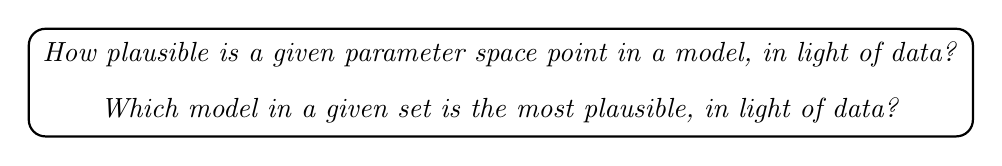
\begin{tikzpicture}
        \node[rectangle, draw, fill = white, rounded corners = 6pt,
          thick, inner sep = 0.5em, align = center]{
          \textit{How plausible is a given parameter space point in a model,
            in light of data?}\\[0.8em]
          \textit{Which model in a given set is the most plausible, in light
            of data?}
        };
      \end{tikzpicture}
    \end{center}
  \item {\color{blue} Rigorous logical framework exists for answering these
    questions: Bayesian statistics}
  \end{itemize}
\end{frame}

\begin{frame}
  \frametitle{Naturalness Priors}
  % - Bayesian approach automatically incorporates intuitions
  %   about naturalness
  % - show derivation of naturalness priors
  % - introduce definition of \Delta_J
  % - summarise merits
\end{frame}

\begin{frame}
  \frametitle{Example: the SM Hierarchy Problem}
  \begin{columns}[t]
    \begin{column}{0.5\textwidth}
      \begin{figure}
        \includegraphics[width=0.9\textwidth]{SM_Lambda}
      \end{figure}
    \end{column}
    \begin{column}{0.5\textwidth}
      \begin{itemize} \itemsep1em
      \item Toy model: $M_Z^2 = -\frac{\bar{g}^2}{8 \lambda} (\mu^2
        + \Lambda_{NP}^2)$
      \item Traditional BG measure applied to, e.g., cut-off $\Lambda_{NP}^2$,
        \begin{equation*}
          \Delta_{\Lambda_{NP}^2} = \frac{\bar{g}^2}{8 \lambda}
          \frac{\Lambda_{NP}^2}{M_Z^2}
        \end{equation*}
        $\Rightarrow$ large tuning for $\Lambda_{NP}^2 \gg M_Z^2$
        \begin{itemize}
        \item But interpretation unclear, e.g., large $\Delta_{\Lambda_{NP}^2}$
          $\equiv$ implausible? When is $\Delta_{\Lambda_{NP}^2}$ too large?
        \end{itemize}
      \item Bayesian approach: posterior for $\Lambda_{NP}^2$ conditioned on
        observed $M_Z^2$, $m_h^2$
      \item Computed in terms of effective ``naturalness prior''
      \end{itemize}
    \end{column}
  \end{columns}
\end{frame}

\section{Results}

\begin{frame}
  \frametitle{Models Considered}
  % - summarise models and methods
\end{frame}

\begin{frame}
  \frametitle{Low Fine-tuning and Credible Regions}
\end{frame}

\begin{frame}
  \frametitle{Impact of $m_h \approx 125$ GeV}
\end{frame}

\begin{frame}
  \frametitle{Comparing Fine-tuning Measures}
\end{frame}

\begin{frame}
  \frametitle{Posterior Distributions}
\end{frame}

\section{Summary}

\begin{frame}
  \frametitle{Summary}
\end{frame}

\appendix

\begin{frame}
  \begin{center}
    {
      \Large
      Additional Slides
    }
  \end{center}
\end{frame}

\end{document}
